\subsection{RQ1: Overall Performance on QA Tasks}
\label{sec:rq1}

\textbf{Software documentation provides essential value for repository comprehension.}
As illustrated in Tables~\ref{tab:rq1_results}, the ``No Doc'' setting (i.e., addressing tasks without inquiring documentation) achieves average performance of only 48.68 and -3.43 in B-ACC and MCC, 30.34 and 28.49 in F1 and IoU, and 18.40 and 20.74 in $\text{EM}_{1.0}$ and $\text{EM}_{0.8}$, respectively. It highlights the challenging nature of \benchmark, where advanced LLMs cannot effectively answer repository-level questions from prior knowledge without consulting the documentation. All six selected methods consistently outperform the ``No Doc'' setting, with absolute improvements ranging from 5.39\% to 16.22\%, 13.03\% to 32.77\%, 17.45\% to 37.95\%, 16.61\% to 36.41\%, 5.97\% to 9.69\%, and 6.39\% to 10.54\% across these six metrics. This directly confirms that documentation offers indispensable value for understanding and locating repository functionalities. 

\textbf{Despite recent advancements, current documentation generation methods still exhibit great limitations.} Our experiments reveal that even top-performance methods struggle to achieve high scores. In functionality detection, the best performance method achieves an average MCC of only 29.35. While performance on functionality localization is relatively higher, with the leading method achieving an average IoU of 64.90, this still implies a notable localization deviation. This limitation is most pronounced in functionality completion, where the leading method scores merely 28.09 and 31.28 on $\text{EM}_{1.0}$ and $\text{EM}_{0.8}$, on average. These results collectively indicate that current automatically generated documentation demonstrates limited navigation ability and struggles to provide comprehensive details. Thus, there is still a gap between current automated methods and practical developer usage.
   
\begin{myfindbox}
    \textbf{Finding 1:} Although documentation aids repository comprehension, the limited performance of current automated methods constrains their practical value for developers.
\end{myfindbox}

\begin{figure*}[t]
	\centering
	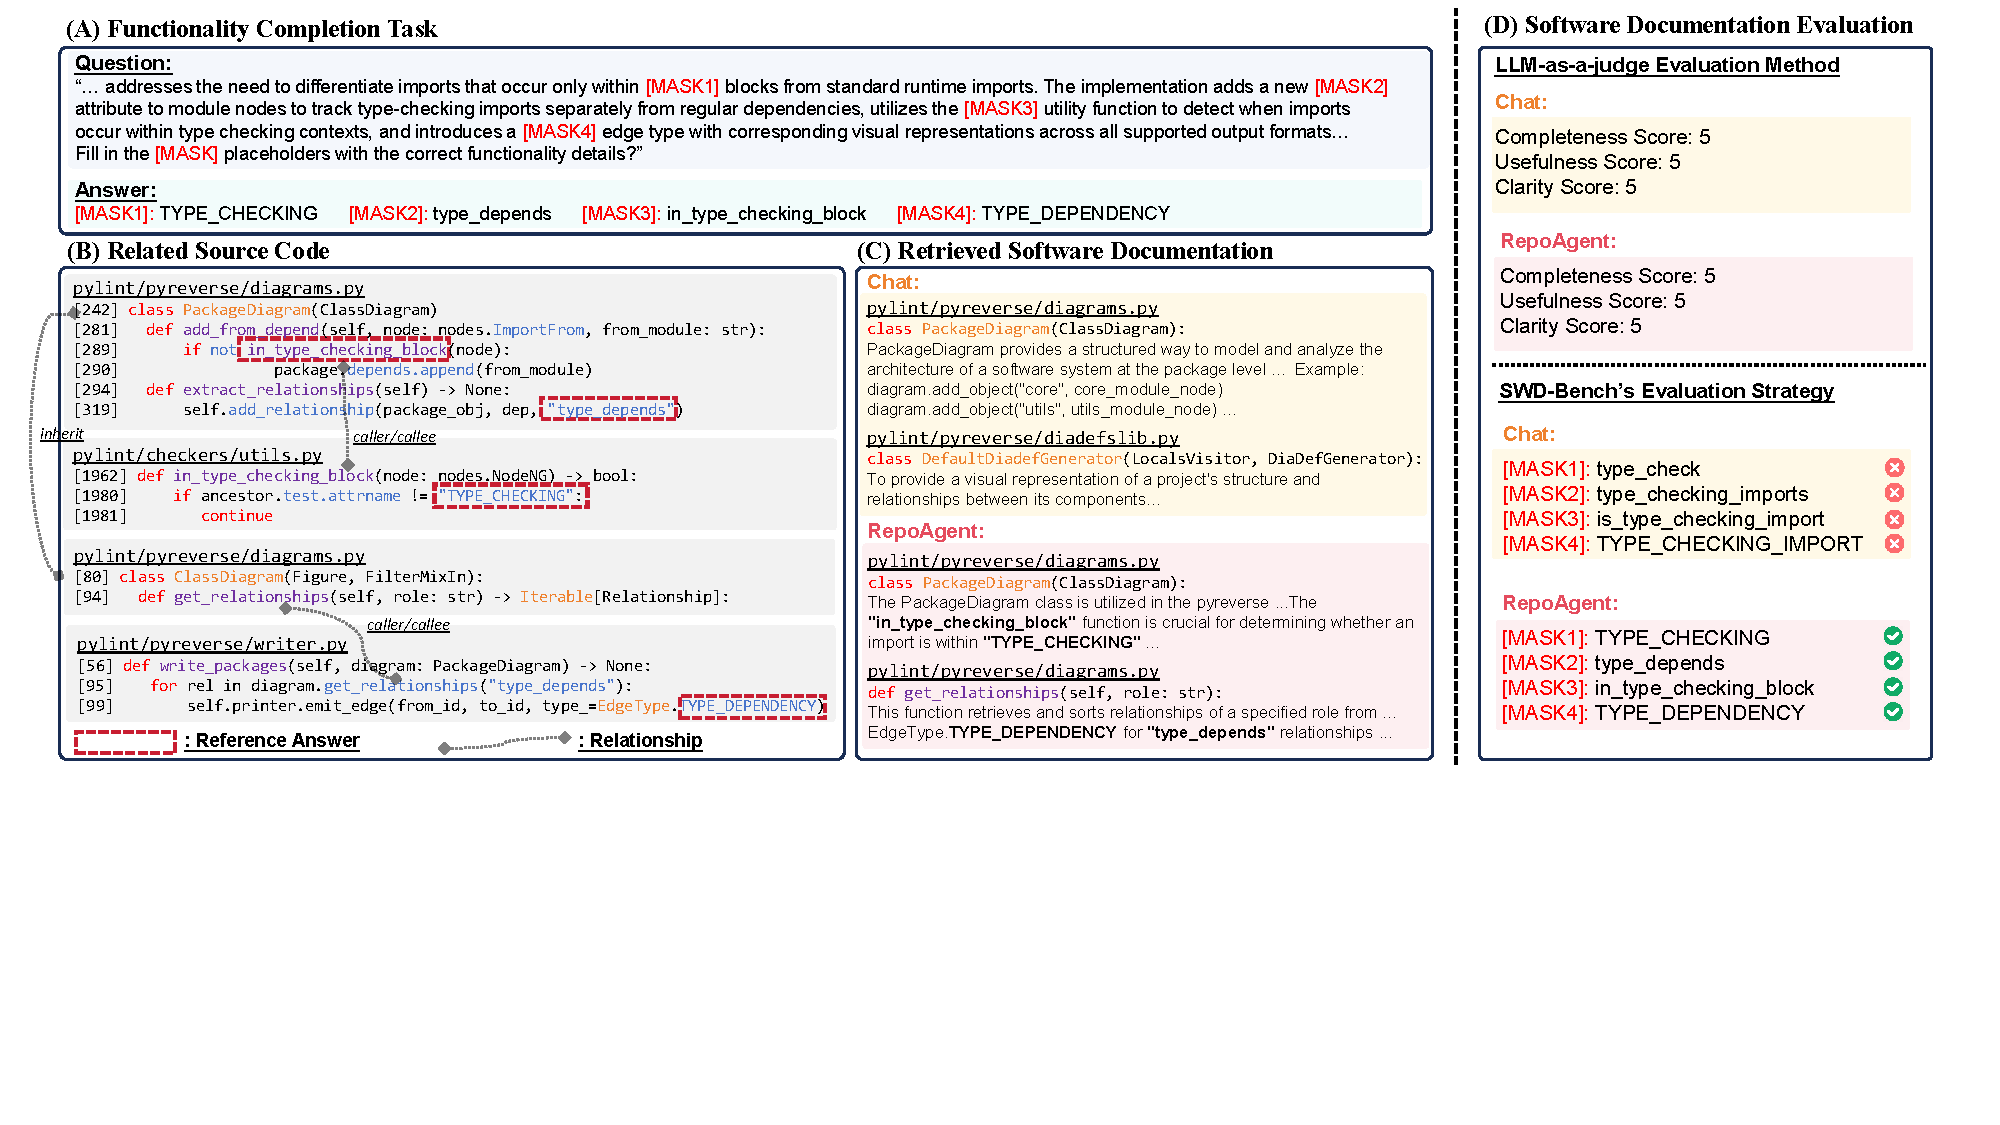
\includegraphics[width=\textwidth]{Figures/case.pdf}
    \vspace{-2.7em}
    \caption{A case study on the functionality detail task (Entry-ID: ``\texttt{pylint-dev/pylint/8824}''). (A) The task question and answer. (B) The related source code to implement the described functionality. (C) The retrieved documentation from Chat and RepoAgent. (D) A comparison of results between the current evaluation method and our evaluation strategy.}
\label{fig:case_study}
\vspace{-1em}
\end{figure*}

\textbf{Fine-grained documentation generation methods achieve superior performance.} We categorize the four repository-level documentation generation methods by their generated documentation granularity: fine-grained (RepoAgent and DocAgent, which focus on code snippets), intermediate-grained (AutoDoc, which operates at the file level), and coarse-grained (DeepWiki, which produces module-level summaries). Overall, fine-grained methods achieve better performance. Specifically, the average performance of RepoAgent and DocAgent relatively improves upon the AutoDoc by 9.45\% and 65.04\% in B-ACC and MCC, 9.59\% and 9.87\% in F1 and IoU, 9.98\% and 8.08\% in $\text{EM}_{1.0}$ and $\text{EM}_{0.8}$. Furthermore, AutoDoc demonstrates a relative improvement over the DeepWiki of 4.04\%, 49.58\%, 26.91\%, 27.19\%, 2.17\%, and 3.34\% on these six metrics. This suggests that fine-grained documentation provides more comprehensive and concrete information, including parameter usage and code examples, which greatly aid in understanding functionality.

\textbf{Integrating global semantic context is crucial for generating high-quality documentation.} Chat, DocAgent, and RepoAgent all generate fine-grained documentation, but they adopt different strategies for integrating global semantic context, resulting in notable performance differences. RepoAgent populates the prompt with comprehensive context using a repository-wide DAG, DocAgent relies on a ``searcher agent'' to retrieve relevant context, and Chat serves as a baseline comparison without context integration. As shown in Tables~\ref{tab:rq1_results}, DocAgent relatively improves upon Chat by 2.86\%, 30.34\%, 3.95\%, 4.02\%, 4.15\%, and 3.56\%, demonstrating that integrating global context directly enhances documentation quality. 
RepoAgent relatively improves upon DocAgent by 11.45\%, 62.27\%, 5.61\%, 6.10\%, 5.32\%, and 6.67\% across the six metrics. This indicates that directly integrating global context into the prompt is a more robust strategy than relying on a sub-agent for retrieving, which may introduce information incompleteness. Besides, H-Written (human-written documentation artifacts) outperform Chat and is even competitive with DocAgent. For instance, its performance on the functionality localization task under the Gemini-2.5-pro model achieves relative improvements of 2.49\% in F1 and 3.43\% in IoU over DocAgent. This result reveals the authentic process of developers' documentation generation, where developers naturally incorporate repository-level context when writing documentation.

\begin{myfindbox}
    \textbf{Finding 2:} Fine-grained methods that utilize comprehensive context deliver stronger performance. Human-written documentation remains competitive, likely because developers naturally incorporate repository-level context.
\end{myfindbox}

\textbf{Extensive documentation-based inquiry enhances deeper repository comprehension.}
To simulate different levels of developer engagement with documentation, we configure three retrieval settings: brief overview (Top 1024 tokens), standard review (Top 2048 tokens), and in-depth inspection (Top 4096 tokens). Our results demonstrate that accessing more documentation information consistently leads to better outcomes. Specifically, transitioning from a brief overview to a standard review, the average performance of six methods relatively improves by 2.71\%, 21.31\%, 4.31\%, 4.10\%, 2.22\%, and 1.65\% on the six metrics. Further expanding to an in-depth inspection yields additional relative improvements of 2.02\%, 11.24\%, 4.03\%, 3.71\%, 1.86\%, and 1.81\%. This trend mirrors the documentation-driven development, where deeper documentation reading results in more accurate repository understanding.

\textbf{\benchmark provides stable evaluation across different foundational models.} Our experiments demonstrate that while the choice of foundational model influences absolute scores, the relative ranking of documentation generation methods remains consistent. Specifically, Gemini-2.5-pro outperforms GPT-4.1 by 5.04\% on B-ACC, 2.57\% on F1, and 2.95\% on $\text{EM}_{1.0}$ on average, likely due to its advanced comprehension capabilities. However, across all methods, RepoAgent consistently ranks first, followed by DocAgent, AutoDoc, and DeepWiki. This indicates that \benchmark can reliably evaluate the documentation under different models. 

\begin{myfindbox}
    \textbf{Finding 3:} Extensive and in-depth documentation-based inquiry enhances repository comprehension. Besides, our evaluation strategy remains stable under different models.
\end{myfindbox}

\subsection{RQ2: Effectiveness of \benchmark's Evaluation Strategy}
We present a case study to demonstrate the advantages of our evaluation strategy over traditional LLM-as-a-judge evaluation. As illustrated in Figure~\ref{fig:case_study}, we select a functionality completion task from \benchmark (Entry-ID: \texttt{pylint-dev/pylint/8824}). The task question (with masked details) and reference answer are presented in Figure~\ref{fig:case_study} (A). Completing this task requires extracting precise and fine-grained information cross multi files. Figure~\ref{fig:case_study} (B) shows the source code for implementing the described functionality, with technical details highlighted in red boxes representing the ground truth for the reference answers. This functionality involves complex cross-file interactions: for example, the ``\texttt{in\_type\_checking\_block}'' function in ``\texttt{utils.py}'' is called by the ``\texttt{add\_from\_depend}'' method in ``\texttt{diagrams.py}'' (line 289), and the ``\texttt{get\_relationships}'' method in ``\texttt{diagrams.py}'' (line 94) is invoked by ``\texttt{writer.py}'' (line 95). Correctly answering the question requires a holistic understanding of these interactions.

Figure~\ref{fig:case_study} (C) displays the retrieved documentation from Chat and RepoAgent. RepoAgent's documentation contains the necessary details (highlighted in bold) to answer the question, due to its integration of global semantic context during generation. For instance, its documentation for the ``\texttt{PackageDiagram}'' class introduces the concept of ``\texttt{TYPE\_CHECKING}'' from the ``\texttt{in\_type\_checking\_block}'' function, and its explanation of ``\texttt{get\_relationships}'' covers the ``\texttt{TYPE\_DEPENDENCY}'' edge type from the ``\texttt{write\_packages}'' function. This context-aware approach enables developers to better understand the implementation and interaction of specific functionalities.
In contrast, Chat's documentation, which lacks repository-level context, produces only generic descriptions with limited guidance. Figure~\ref{fig:case_study} (D) illustrates the results of two different evaluation strategies. The LLM-as-a-judge method assesses the documentation on dimensions like ``Completeness'' and ``Usefulness''. Since the LLM lacks prior knowledge of the repository, it can only evaluate surface-level quality. As a result, it awards both documentation a perfect score of 5, failing to distinguish their practical value. In contrast, \benchmark's evaluation strategy, based on repository-level QA tasks, reveals clear differences: RepoAgent correctly fills the four masked placeholders, while Chat fails on all of them. This case study demonstrates that our evaluation strategy can assess the practical guidance of software documentation for development.

\begin{myfindbox}
    \textbf{Finding 4:} Compared to current evaluation methods, our evaluation strategy based on functionality-driven QA tasks can provide an accurate assessment of documentation quality. 
\end{myfindbox}

\subsection{RQ3: Impact of Documentation Quality on Issue Solving}

In this RQ, we investigate the impact of documentation quality on issue solving. Based on the selected version in Section~\ref{sec:repo_selection}, we collect 57 corresponding instances from the SWE-Bench Verified~\cite{swebench} and adopt SWE-Agent~\cite{swe-agent} as a representative issue-solving method. For each instance, we provide SWE-Agent with retrieved software documentation (Top 4096 tokens) based on the issue description. The results are shown in Figure~\ref{fig:discussion}. 

\textbf{Software documentation can help improve issue-solving performance.} The baseline issue-solving rate of SWE-Agent (retrieving from the code repository) is 43.86\%. When documentation is provided, the relative issue-solving improvement ranges from 8.00\% to 20.00\%, with the issue file location rates improving by 6.01\% to 11.19\%. These enhancements can be attributed to the global information and complementary context provided in the documentation, which helps SWE-Agent locate and address issues. 

\textbf{Higher-quality documentation provides greater benefits in issue-solving.} The performance ranking of four repository-level documentation generation methods observed in RQ1—with RepoAgent ranks highest, followed by DocAgent, AutoDoc, and DeepWiki—is similarly reflected in the issue-solving results. Specifically, RepoAgent achieves the highest issue-solving rate at 52.63\%, followed by DocAgent and AutoDoc, both at 49.12\%, and DeepWiki at 47.37\%. This consistency demonstrates that our evaluation strategy is effective for evaluating documentation, as higher-quality documentation aids in solving real-world issues.

\begin{figure}[t]
    \centering
    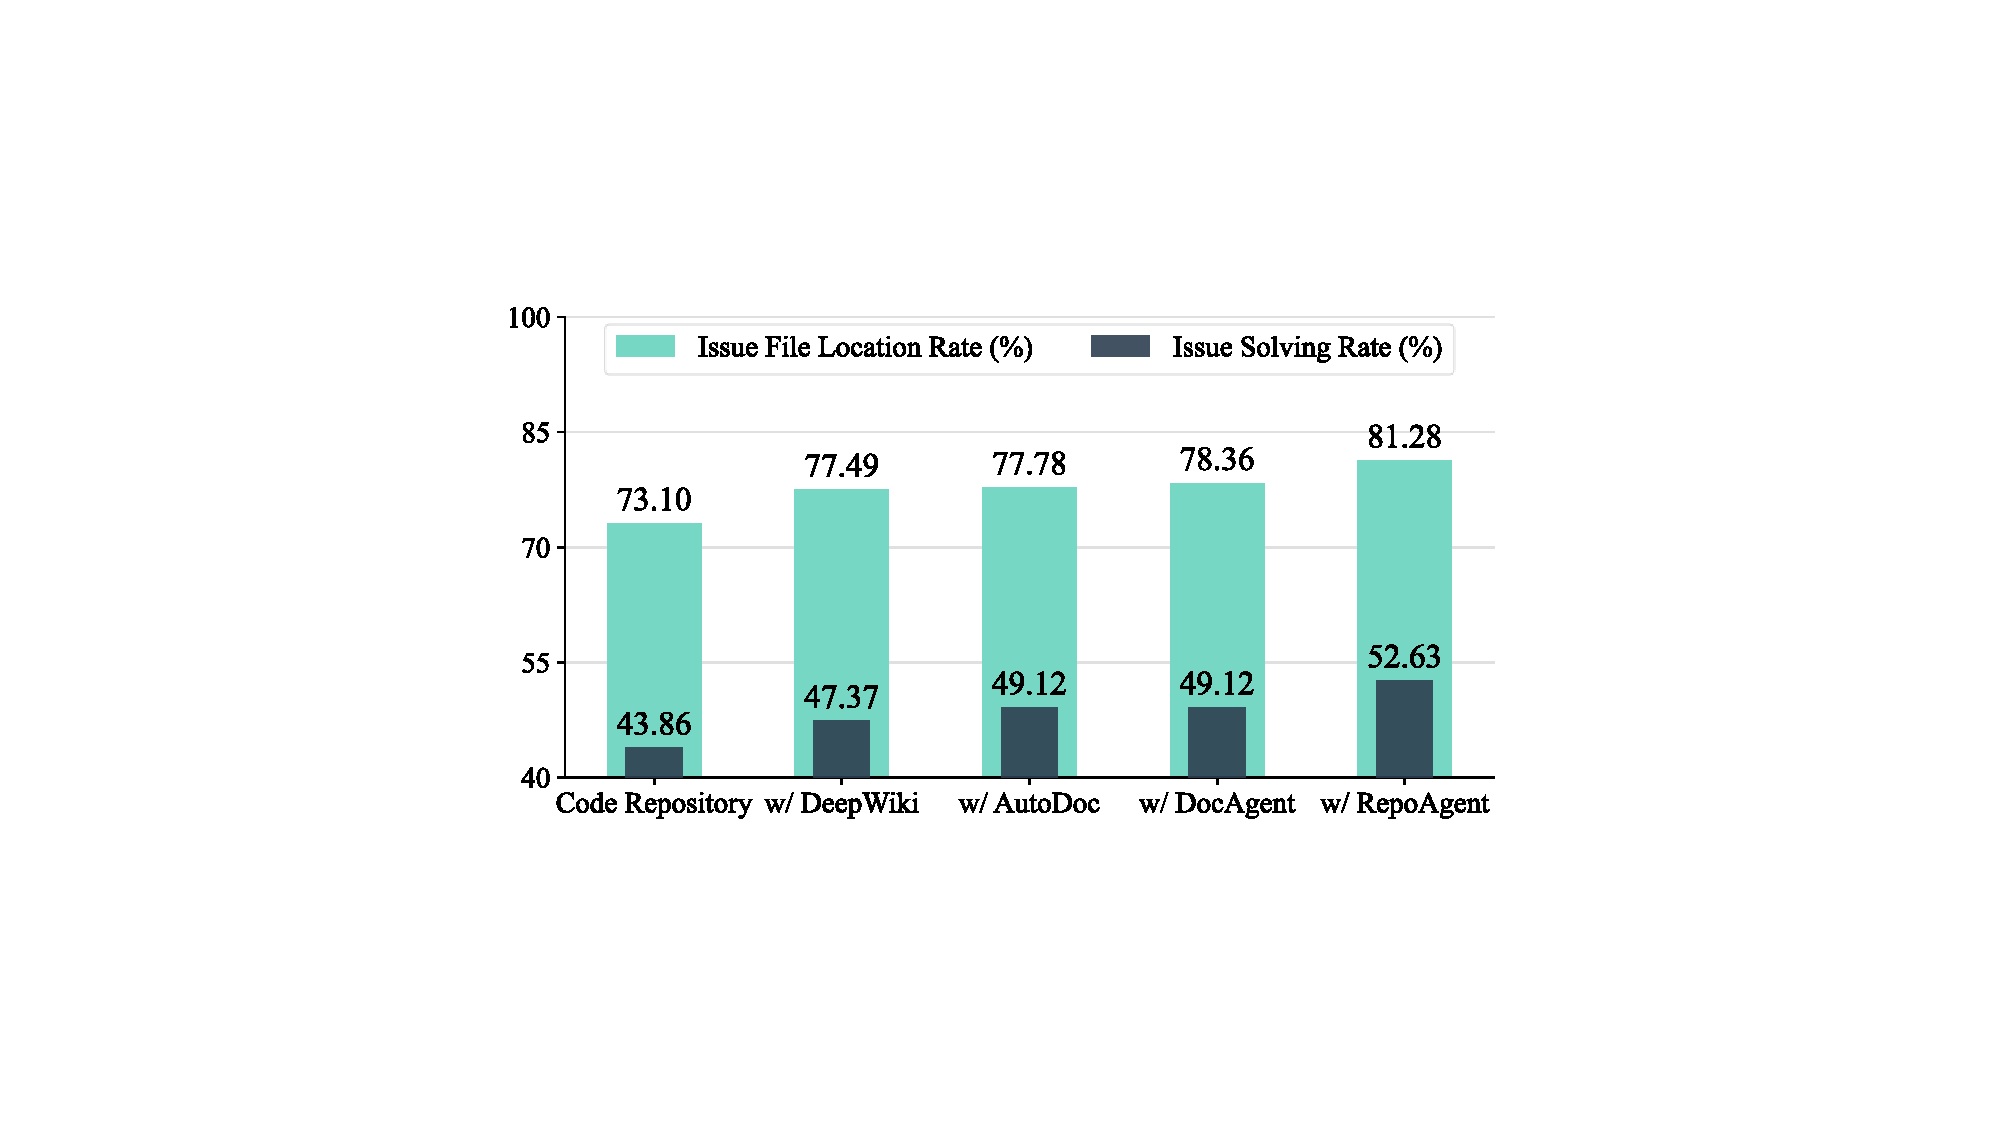
\includegraphics[width=.45\textwidth]{Figures/discussion.pdf}
    \vspace{-1.2em}
    \caption{Performance of SWE-Agent on issue solving when provided with different software documentation.}
    \label{fig:discussion}
    % \vspace{-1.5em}
\end{figure}

\begin{myfindbox}
\textbf{Finding 5:} Higher-quality software documentation is more conducive to issue solving, highlighting its practical value in supporting documentation-driven development.
\end{myfindbox}

